One of the most popular knowledge graphs is Freebase~\cite{Bollacker2008FreebaseAC}. Although it is not maintained anymore since it was integrated into Wikidata in 2015~\cite{Tanon2016FromFT}, the benchmark datasets derived from it are still widely used. One of those benchmark datasets is the \emph{FB15k} dataset introduced by Bordes et al. in 2013~\cite{Bordes2013TranslatingEF}, which covers roughly \num{15000} Freebase entities. On its basis, Toutanova and Chen introduced the FB15k-237 subset in 2015~\cite{Toutanova2015ObservedVL}, whose purpose was to create a more meaningful benchmark by eliminating trivially predictable facts. For example, if FB15k-237 covers a relation like $(x, contains, y)$, it does not include its inverse relation $(y, part~of, x)$, because good performance resulting from such trivial, mutual predictions detracts from more interesting cases. In 2020, Safavi and Koutra published another dataset called CoDEx~\cite{Safavi2020CoDExAC}, which is derived from FB15k-237 and two other datasets, covers more diverse content and in turn poses a greater challenge than FB15k and FB15k-237. From the three provided variants of the CoDEx dataset -- CoDEx-S, CoDEx-M, and CoDEx-L -- the IRT approach by Hamann, on which this work is based, focuses on the CoDEx-M dataset. \autoref{tab:5_experiments/1_data_sources/1_knowledge_graphs/benchmark_datasets} gives an overview of the scales of FB15k, FB15k-237 and CoDEx-M. CoDEx-M actually contains additional, negative facts that are excluded here as this work focuses on the common open-world scenario.

\begin{table}[h]
    \centering
    \begin{tabular}{| l | r | r | r | r | r |}
    \hline

    \multicolumn{1}{|c|}{\textbf{Dataset}} &
    \multicolumn{1}{|c|}{\textbf{#Entities}} &
    \multicolumn{1}{|c|}{\textbf{#Relations}} &
    \multicolumn{3}{|c|}{\textbf{#Facts}} \\

    \multicolumn{1}{|c|}{} &
    \multicolumn{1}{|c|}{} &
    \multicolumn{1}{|c|}{} &
    \multicolumn{1}{|c|}{\textbf{Train}} &
    \multicolumn{1}{|c|}{\textbf{Valid}} &
    \multicolumn{1}{|c|}{\textbf{Test}} \\

    \hline \hline

    FB15k     & \num{14951} & \num{1345} & \num{483142} & \num{50000} & \num{59071} \\
    FB15k-237 & \num{14541} & \num{237}  & \num{272115} & \num{17535} & \num{20466} \\
    CoDEx-M   & \num{17050} & \num{51}   & \num{185584} & \num{10310} & \num{10311} \\

    \hline
\end{tabular}

    \caption{Comparison of popular KGC benchmark datasets}
    \label{tab:5_experiments/1_data_sources/1_knowledge_graphs/benchmark_datasets}
\end{table}

As for the above KGC benchmark datasets, a graph's fact set is usually further split into training, validation, and test subsets. Thereby, the splits are created so that there are training, validation, and test facts for possibly every entity. In contrast to that common approach, in his work on zero-shot learning, Hamann creates new \emph{IRT splits} from FB15k-237 and CoDEx-M that distinguish between so-called \emph{closed-world (CW) entities}, that are seen during training, and \emph{open-world (OW) entities}, which are not seen during training, to optimize prediction for unknown entities.

\begin{figure}
    \centering
    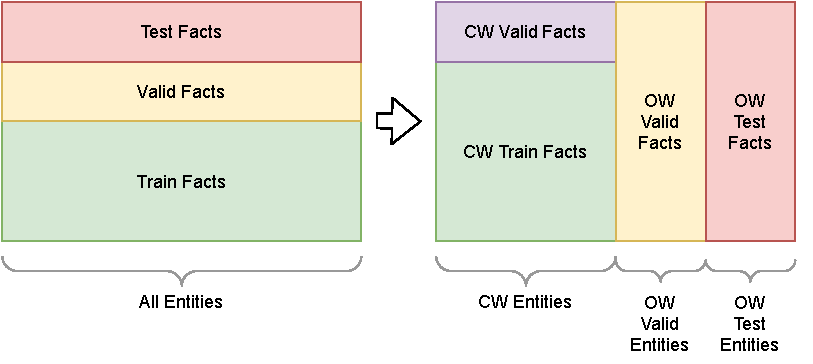
\includegraphics[width=\textwidth]{5_experiments/1_data_sources/1_knowledge_graphs/irt_split}
    \caption{Difference between a conventional and an IRT fact split. The IRT fact split focuses on open-world entities that must stay unseen during training. ``CW'' = ``closed-world'', ``OW'' = ``open-world''.}
    \label{fig:5_experiments/1_data_sources/1_knowledge_graphs/irt_split}
\end{figure}

\autoref{fig:5_experiments/1_data_sources/1_knowledge_graphs/irt_split} illustrates the different shape of an IRT fact split compared to a conventional one: The closed-world entities' facts are split into closed-world training and closed-world validation facts to enable closed-world prediction. Meanwhile, the open-world entities' facts are completely reserved for validation and training, respectively. Closed-world training and closed-world validation facts only refer to closed-world entities. On the other hand, one of an open-world validation fact's head or tail may also be a closed-world entity, and one of an open-world test fact's head or tail may be a closed-world entity or an open-world validation entity. \autoref{tab:5_experiments/1_data_sources/1_knowledge_graphs/irt_splits} gives an overview of the scales of the IRT splits' entity and fact subsets.

\begin{table}[h]
    \centering
    \begin{tabular}{ l c r r r c r r c r r }
    \toprule
    
    \multicolumn{1}{l}{\textbf{Graph}} & \phantom &
    \multicolumn{1}{c}{\textbf{\thead{CW \\ Train \\ Ents}}} &
    \multicolumn{1}{c}{\textbf{\thead{CW \\ Train \\ Facts}}} &
    \multicolumn{1}{c}{\textbf{\thead{CW \\ Valid \\ Facts}}} & \phantom &
    \multicolumn{1}{c}{\textbf{\thead{OW \\ Valid \\ Ents}}} &
    \multicolumn{1}{c}{\textbf{\thead{OW \\ Valid \\ Facts}}} & \phantom &
    \multicolumn{1}{c}{\textbf{\thead{OW \\ Test \\ Ents}}} &
    \multicolumn{1}{c}{\textbf{\thead{OW \\ Test \\ Facts}}} \\

    \midrule

    FB15k-237 && \num{12057} & \num{214412} & \num{23778} && \num{1545} & \num{46503} && \num{816}  & \num{25423} \\
    CoDEx-M   && \num{11399} & \num{123650} & \num{13738} && \num{2918} & \num{41240} && \num{1896} & \num{27577} \\

    \bottomrule
\end{tabular}

    \caption{Scale of the IRT splits of the FB15k-237 and CoDEx-M datasets}
    \label{tab:5_experiments/1_data_sources/1_knowledge_graphs/irt_splits}
\end{table}
